\chapter{Research Methodology}
\section{Introduction}
This chapter discusses how the research is executed. An overview of the research methodology is provided in the research framework. The dataset and software used in conducting the experiments are explained in detail. The general approach on how AS models are constructed and evaluated is also discussed. 

\section{Research Framework}
\label{sec:researcframework}
The study underwent through four phases: \textit{Identify Research Problem}, \textit{Prepare Development Environment}, \textit{Build and Evaluate AS Model}, and \textit{Present Results}. The research flow is illustrated in Figure \ref{fig:researchframework}.

\begin{figure}[H]
	\centering
	\scalebox{.6}{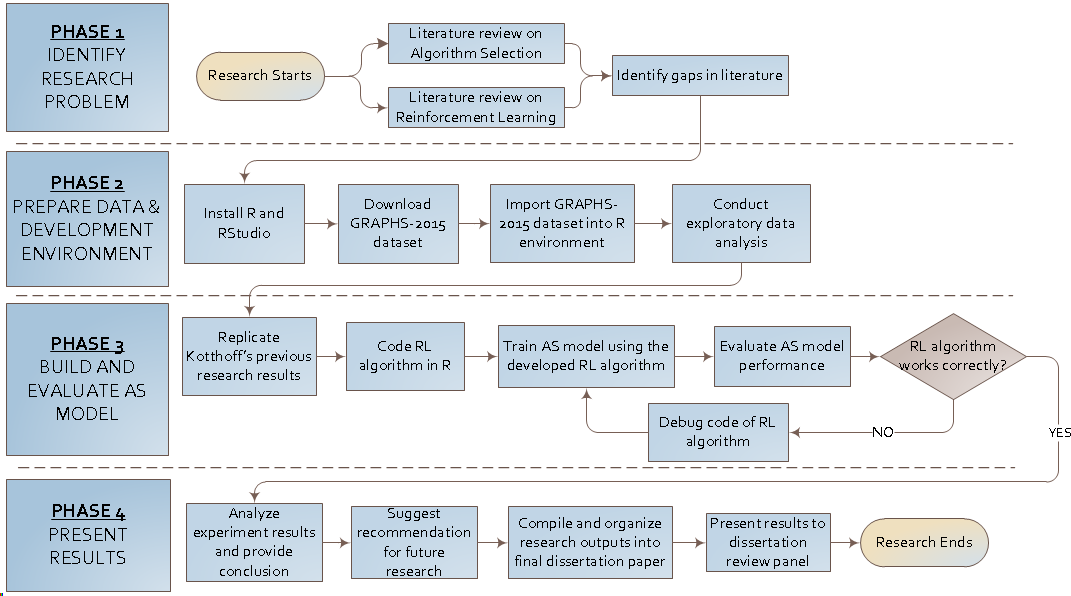
\includegraphics{./img/research_framework.png}}
	\caption{Research Framework} 
	\label{fig:researchframework}
\end{figure}

\section{Phase 1: Identify Research Problem} 
This research is inspired by the Open Algorithm Selection Challenge 2017 \citep{lindauer2017open} which showcased the latest techniques in AS. The datasets and tools used in the challenge have been made publicly available, allowing anyone to easily replicate the results. This lowers the barrier to entry to AS research.

The AS survey papers by Kotthoff \citep{kotthoff2016portfolios} and Smith-Miles \citep{smith2009cross} served as starting point in learning the background of AS. This study decided to focus on the application of AS to subgraph isomorphism problems. It has been chosen since a recent study of the same topic by Kotthoff and his colleagues \citep{kotthoff2016algorithm} published data and results that can be easily reproduced. This study is referred to a number of times in this paper and will henceforth abbreviated to PORTSUB for convenience. This study follows up on PORTSUB by proposing RL as an alternative in training AS models.

\section{Phase 2: Prepare Data and Development Environment} 
The experiments are executed on a server class desktop running Ubuntu Server 16.04 with 16 Gb RAM, Intel Xeon 4.0 GHz 12-core CPU, and an nVidia GeForce GTX1080Ti GPU. Experiments also ran well on a laptop installed with Windows 7 with 16 Gb RAM and Intel i7 3.0 GHz quad-core CPU. It is not really necessary to run the experiments on machines with specs as high as described since the computational requirements of training the AS models in this study are not very demanding. The experiments can be decently conducted on a Windows, MacOS, or GNU/Linux system with at least 4 Gb RAM and a 2.5 GHz quad-core CPU. 

\subsection{Install Development Software and Libraries}
All experiments are executed in R. R is a programming language for statistical computing and graphics. R’s capabilities suit well the experimental needs of this research, which include mostly data handling, data analysis, and plotting results. To develop in R, using an IDE such as RStudio is recommended. RStudio is an integrated set of tools that helps one to be more productive with R.

\begin{figure}[H]
	\centering
	\scalebox{.6}{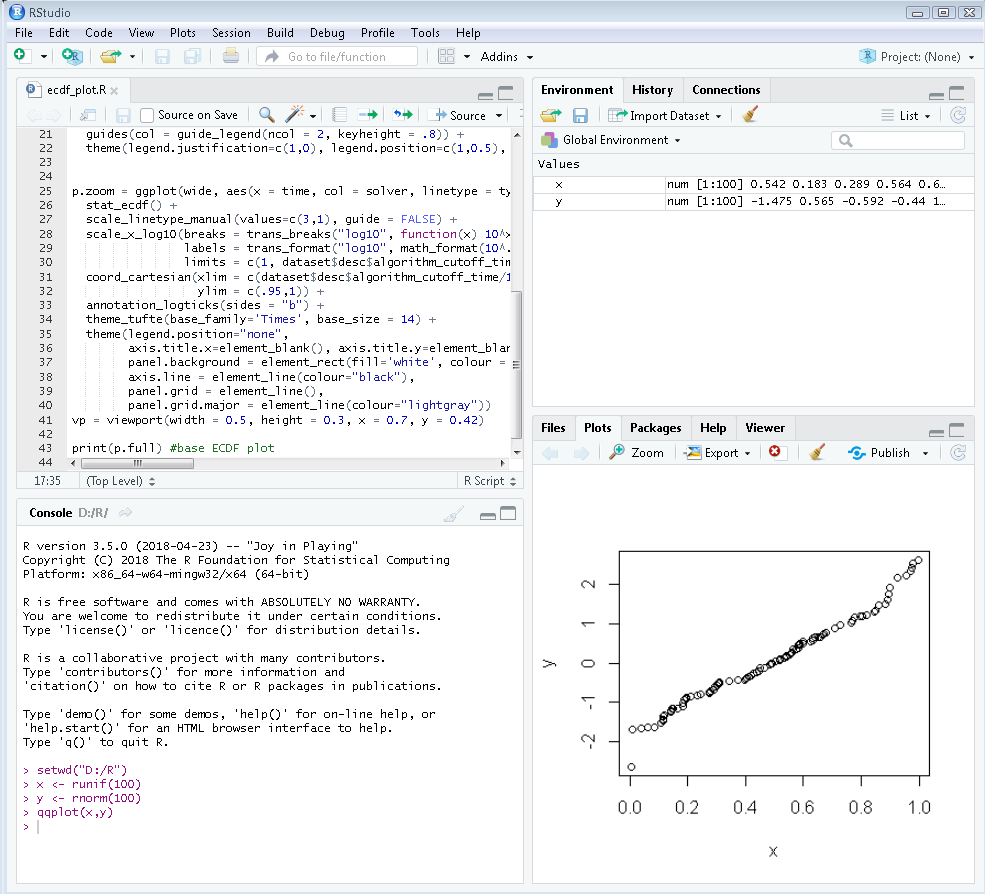
\includegraphics{./img/rstudio.png}}
	\caption{RStudio IDE} 
	\label{fig:rstudio}
\end{figure}

Libraries in R are called \textit{packages}. Packages bundle together code, data, documentation, and tests, and is easy to share with others \citep{wickham2015r}. Two R packages developed especially for AS research are available: these are ASlib and LLAMA.

\begin{figure}[H]
	\centering
	\scalebox{.8}{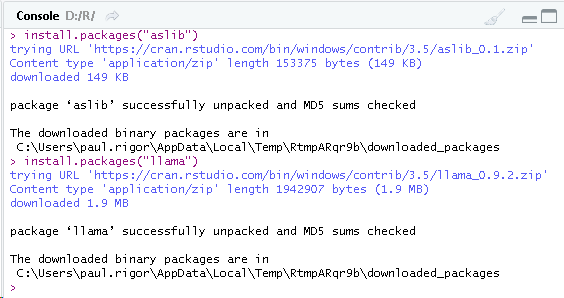
\includegraphics{./img/install_packages.png}}
	\caption{Installing packages in R} 
	\label{fig:installpackages}
\end{figure}

\subsubsection{Algorithm Selection Library (ASlib)}
Algorithm Selection Benchmark Library (ASlib) is an R package for operating on and analyzing AS datasets. This package allows researchers to work on AS problems and perform reproducible comparisons of approaches \citep{bischl2016aslib}. An ASlib dataset is called an \textit{AS scenario}. This contains pre-computed results for an algorithm portfolio on a set of problem instances, i.e., the performance measure is known for all pairs of algorithms and instances. In addition, the set of pre-computed instance features and its associated costs (the time spent in computing a feature) is provided for each instance. Providing this information makes it easy to build AS models, which typically involves (1) generating problem instances, (2) constructing an algorithm portfolio, (3) coding the algorithms, and (4) building the AS model. ASlib enables researchers to focus on (4) by providing the necessary data on (1) - (3). Furthermore, ASlib allows a fair and convenient evaluation and comparison of algorithm selectors.

The basic structure of an ASlib scenario is shown on \ref{tbl:aslibscenario}. The complete specification can be found online \citep{aslibspec}.

\begin{table}[H]
	\centering
	\begin{tabulary}{\textwidth}{|l|l|L|}
		\hline
		\multicolumn{1}{|c|}{\textbf{File Type}} & \multicolumn{1}{c|}{\textbf{Filename}} & \multicolumn{1}{c|}{\textbf{Description}} \\ \hline
		Meta information file & description.txt & Global description file containing general information about the scenario, including the name of the scenario, performance measures, algorithms, features and limitations of computational resources. \\ \hline
		Algorithm performance & algorithm\_runs.arff & Contains performance measurements with possible repetitions and completion status of the algorithm runs. The performance metric can be arbitrary, e.g., runtime, solution quality, accuracy or loss. \\ \hline
		Instance feature & feature\_values.arff & Contains the feature vectors for all instances. \\ \hline
		Feature costs & feature\_costs.arff & Contains the costs of the feature groups, i.e., sets of features computed together. \\ \hline
		Cross validation & cv.arff & Describes how to split the instance set into training and test sets to apply a standard machine learning approach to obtain an unbiased estimate of the performance of an algorithm selector. \\ \hline
	\end{tabulary}
	\caption{Basic structure of an ASlib scenario}
	\label{tbl:aslibscenario}
\end{table}


\subsubsection{Leveraging Learning to Automatically Manage Algorithms (LLAMA)}

Several previous studies implement AS models using different software environments like MATLAB and C++. Moreover, the implementations are highly tuned and customized for a particular problem domain. The Leveraging Learning to Automatically Manage Algorithms (LLAMA) R package addresses this problem by providing a common infrastructure for researchers to build, evaluate, and apply AS models \citep{kotthoff2013llama}. 

At a high level, LLAMA takes problem features and algorithm performance data as input (imported to R using ASlib package), feeds it to the AS model, and then outputs the model performance results. LLAMA contains built-in AS model training algorithms; it also allows custom ones to be implemented. Lastly, built-in performance measures in LLAMA include number of solved problems, misclassification penalty (MCP), and penalized average runtime (PAR) score.

\begin{figure}[H]
	\centering
	\scalebox{.8}{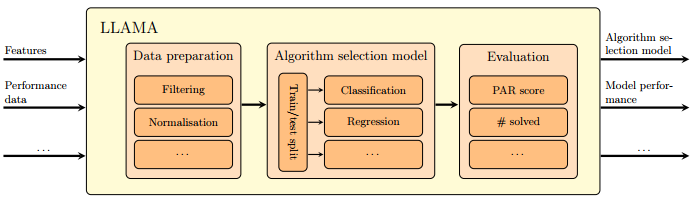
\includegraphics{./img/llama.png}}
	\caption{LLAMA framework}
	\label{fig:llama}
\end{figure}

\subsection{Prepare Dataset}
PORTSUB published a dataset called GRAPHS-2015, which is used to train and test the AS models in this study. It is available online in GitHub \citep{graphs2015} and is currently maintained by the Configuration and Selection of Algorithms (COSEAL) group.

\begin{figure}[H]
	\centering
	\scalebox{.6}{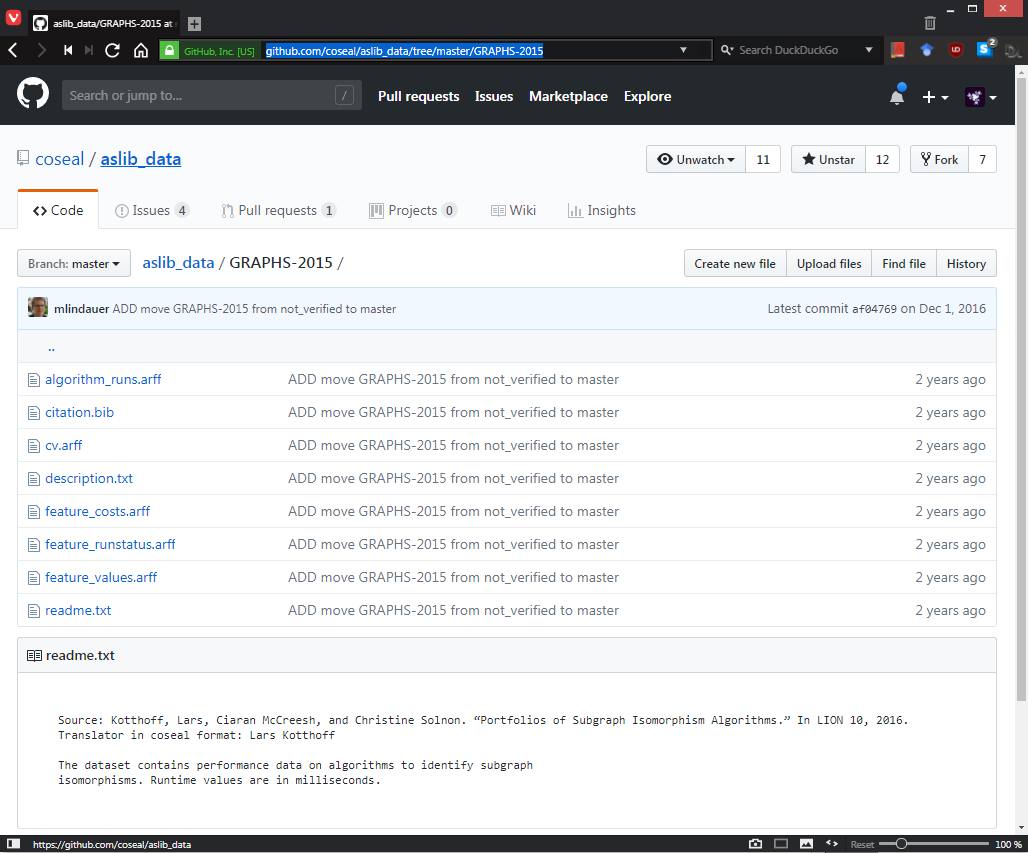
\includegraphics{./img/graphs2015github.png}}
	\caption[GRAPHS-2015 GitHub page]{GRAPHS-2015 GitHub page.}
	\label{fig:graphs2015github}
\end{figure}

\subsection{Replicate Previous Research Results}
The results of PORTSUB are replicated to verify its validity and to later serve as reference for benchmarking the AS model trained using RL. PORTSUB used a supervised learning technique called pairwise random forest regression (PRFR) to train an AS model in solving subgraph isomorphism problems. An implementation of this algorithm is readily available in LLAMA.

\section{Phase 3: Build and Evaluate AS Model}

An AS model is constructed in R, using the ASlib and LLAMA libraries to load the dataset and perform evaluation. The RL algorithm REINFORCE is studied and applied to AS of subgraph isomorphism problems. Its implementation utilized several functions found from the TensorFlow R package. TensorFlow is an open-source machine learning library used for high performance numerical computation \citep{abadi2016tensorflow}.

The effectiveness of AS is determined by comparing its performance against the virtual best solver (VBS) and the single best solver (SBS). VBS is the hypothetical model that does perfect AS, i.e., it always selects the best algorithm for each problem. SBS is the one algorithm from the algorithm portfolio that has the overall best performance across a set of problems. VBS defines the theoretical upper-bound performance that can be achieved by an AS model, while SBS defines the lower-bound performance. An AS model should at least get better performance than SBS to prove that AS is more effective than a single algorithm approach. An AS model becomes more effective as its performance gets closer to the VBS.

An AS model can be evaluated by its ability of how often it assigns the most optimal algorithms to a set of problems. In this study, the AS model performance is measured by calculating the mean misclassification penalty (MCP). This metric represents the additional time spent in solving problems when suboptimal algorithms were chosen. Individual algorithm performance is measured by its runtime, which is defined as the time taken by an algorithm to solve a problem instance. 

VBS, by its definition, always have mean MCP equal to zero. Lower MCP values signify better AS model performance. 


\begin{equation}
MCP = \frac{1}{N}\sum_{i=1}^{N}(t_{S_{i}} - t_{VBS_{i}})
\label{eq:mcp}
\end{equation}

where:

\begin{table}[H]
	\centering
	\begin{tabular}{rl}
		$N =$ & Total number of problem instances \\
		$t_{S_i} =$ & Runtime of the algorithm selected by the AS model \\
		$t_{VBS_i} =$ & Runtime of the algorithm selected by the VBS \\
		$i =$ & \textit{ith} problem instance
	\end{tabular}
\end{table}

\section{Phase 4: Present Results}

The last phase of this study compiles and organizes the findings into a full dissertation paper. The experiment results are discussed and conclusions are made. Lastly, recommendations for future research is presented.